\part{Non-toric singularities}

    \begin{figure}[H]
        \centering
        %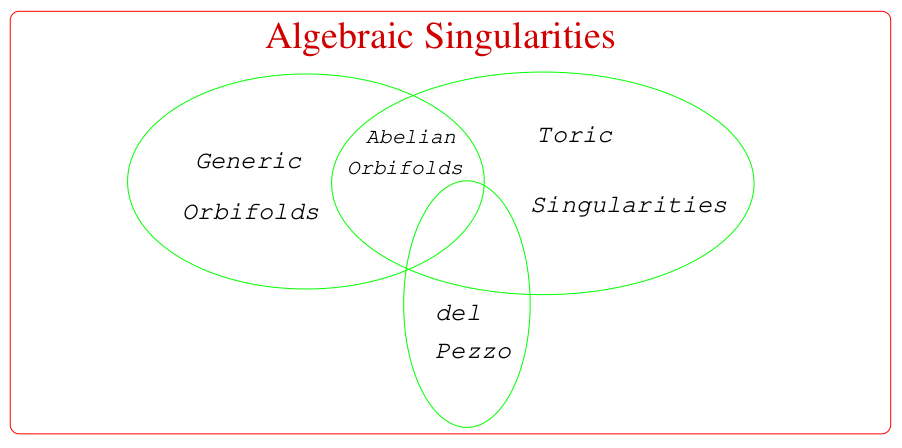
\includegraphics[scale=0.3]{Pictures/algebraicsingularities.png}
        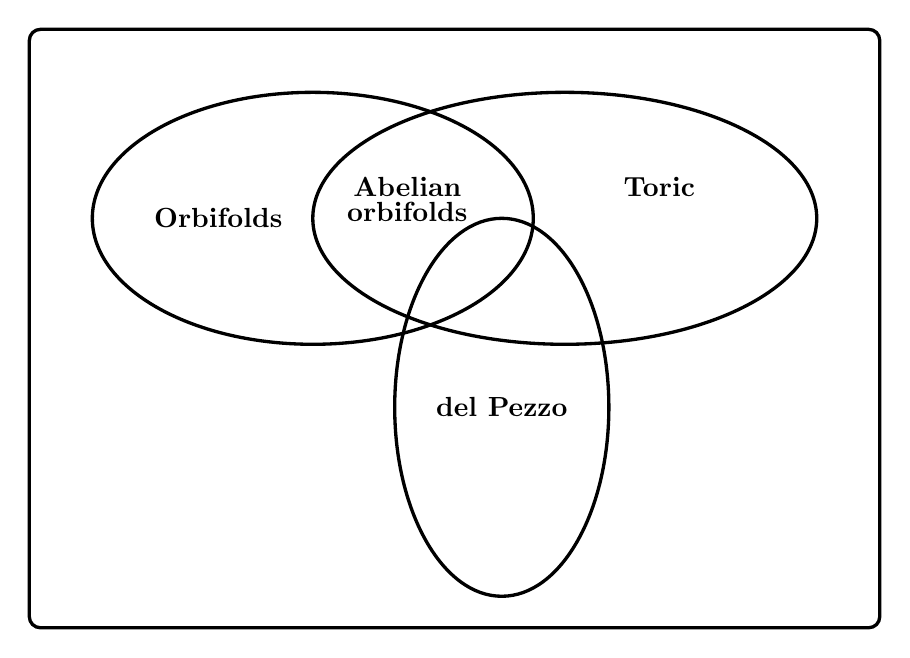
\begin{tikzpicture}[scale=0.8]
            \draw[very thick] (0,3) ellipse (3.5cm and 2cm);
            \draw[very thick] (4,3) ellipse (4cm and 2cm);
            \draw[very thick] (3,0) ellipse (1.7cm and 3cm);
            \draw[rounded corners,very thick] (-4.5, -3.5) rectangle (9, 6) {};
            \draw (-1.5,3) node[]{\textbf{Orbifolds}};
            \draw (1.5,3.5) node[]{\textbf{Abelian}};
            \draw (1.5,3.1) node[]{\textbf{orbifolds}};
            \draw (5.5,3.5) node[]{\textbf{Toric}};
            \draw (3,0) node[]{\textbf{del Pezzo}};
        \end{tikzpicture}
        \caption{Venn diagram of different types of algebraic singularities.}
    \end{figure}

\section{Non-commutative resolutions}
